\documentclass{article}
\usepackage[margin=0.5in]{geometry}
\usepackage{amsmath}
\usepackage{graphicx}
\usepackage{amssymb}
\usepackage{multicol}
\usepackage{xcolor}
\usepackage{amsthm}
\usepackage{mdframed}
\usepackage{tikz}


\newenvironment{tightcenter}{%
    \setlength\topsep{0pt}
    \setlength\parskip{0pt}
    \begin{center}
}{%  
    \end{center}
}
\newcommand{\R}{\mathbb{R}}
\newcommand{\Z}{\mathbb{Z}}
\newcommand{\C}{\mathbb{C}}
\newcommand{\K}{\mathbb{K}}
\newcommand{\PP}{\mathbb{P}}
\newcommand{\E}{\mathcal{E}}
\newcommand{\e}{\vspace{3mm}}
\title{Práctica 1 - Experimentos aleatorios. Espacio muestral; eventos}
\author{Santiago}
\date{}
\begin{document}
    \maketitle
    \global\mdfdefinestyle{s}{%
            linecolor=orange,linewidth=0.5pt,%
            leftmargin=0cm,rightmargin=1cm
        }
    \begin{enumerate}
        \item Asociar un espacio muestral a cada uno de los siguientes experimentos aleatorios.
    \begin{enumerate}
        \item Lanzar tres veces al aire una moneda y observar el lado que cae hacia arriba.
            \begin{mdframed}[style=s]
                El espacio muestral es el conjunto de resultados posibles de un experimento. En este caso particular, al tirar una moneda la misma puede caer con cara o cruz hacia arriba. Podemos denotar los siguientes eventos:
                \begin{center}
                    A: Sale cara\\
                    B: Sale cruz
                \end{center}
                Entonces tenemos que:\[\Omega=\{AAA,AAB,ABA,ABB,BAA,BBA,BAB,BBB\}\]
            \end{mdframed}
        \item Lanzar tres veces al aire una moneda y observar el número total de caras.
            \begin{mdframed}[style=s]
                Puede suceder que en los tres tiros no salga cara, también puede caer una vez, dos veces, e incluso tres. Por lo tanto:\[\Omega=\{0,1,2,3\}\]
            \end{mdframed}
        \item Una urna contiene 2 bolillas blancas y una negra. Se sacan 2 bolillas al azar simultáneamente y se anotan los colores.
            \begin{mdframed}[style=s]
                Como estoy anotando los colores, no se distingue entre las dos bolillas blancas. Considerando los eventos
                \begin{center}
                    N: negra\\
                    B: blanca
                \end{center}
                se tiene que\[\Omega=\{BB,BN\}\]
            \end{mdframed}
        \item Idem que en el inciso anterior pero con reemplazo.
            \begin{mdframed}[style=s]
                En este caso, al poder reemplazar, está la posibilidad de sacar dos veces la negra.\[\Omega=\{BB,BN,NN\}\]
                Hay que dintinguir entre sacar blanco-negro y negro-blanco?
            \end{mdframed}
        \item Se colocan al azar tres bolillas diferentes en tres urnas diferentes, pudiéndose poner más de una bolilla por urna.\vspace{3mm}\\
            Si representamos cada resultado como \[(U_{B_1},U_{B_2},U_{B_3})\]
            siendo $U_{B_i}$ la urna en donde se encuentra la bolilla $i$. Entonces
            \begin{center}
                $\Omega=\{(1,1,1),(1,1,2),(1,1,3),(1,2,1),(1,2,2),(1,2,3),(1,3,1),(1,3,2),(1,3,3),$\\
                $(2,1,1),(2,1,2),(2,1,3),(2,2,1),(2,2,2),(2,2,3),(2,3,1),(2,3,2),(2,3,3),$\\
                $(3,1,1),(3,1,2),(3,1,3),(3,2,1),(3,2,2),(3,2,3),(3,3,1),(3,3,2),(3,3,3)\}$
            \end{center}
            Como hay un número considerable de resultados, quizás es más conveniente expresar el espacio muestral por comprensión:
            \[\Omega=\{(i,j,k):i,j,k=1,2,3\}\]
        \item Se arroja una moneda; si sale cara se arroja un dado, si sale ceca se lanzan dos dados.\vspace{3mm}\\
            Si denominamos los siguientes eventos:
            \begin{center}
                A: cara\\
                B: ceca
            \end{center}
            \[\Omega=\{(A,i):i\in\mathbb{N}/i<7\}\cup\{(B,i,j):i,j=1,2,3,4,5,6\}\]
        \item Un viajante debe visitar cinco ciudades y traza su itinerario.\vspace{3mm}\\
            Supongamos que las ciudades las enumeramos del 1 al 5.\[\Omega=\{i_1,i_2,i_3,i_4,i_5:i_k\in[1;5],i_m\neq i_n\forall m\neq n\}\]
        \item Los artículos provenientes de una línea de producción se clasifican en defectuosos (D) y no defectuosos (N). Se observan artículos y se anota su condición. Este proceso se continúa hasta que se produzcan dos artículos defectuosos consecutivos o hasta que se hayan verificado cuatro artículos cualesquiera.
            \[\Omega=\{DD,NDD,NNDD,DNDD,DNDN,DNND,DNNN,NNNN,NDND,NDNN,NNDN,NNND\}\]
        \item Una caja con 12 lámparas tiene 4 unidades con filamentos rotos. Se las prueba hasta que se encuentre una
        quemada.\vspace{3mm}\\
            Definimos los eventos:
            \begin{center}
                Q: quemada\\
                N: no quemada
            \end{center}
            Entonces,
            \[\Omega=\{N^iQ:0\leq i\leq8\}\]
        \item Un tanque de agua tiene una bomba cuyo motor se pone en funcionamiento automáticamente cuando el consumo
        hace que el volumen de agua baje hasta cierto nivel. Supongamos que esto puede ocurrir a lo sumo una vez al
        día. Cierto día se observa el motor durante 24 horas y se registra en qué instante ha comenzado a funcionar o
        si no lo ha hecho en todo el día.\vspace{3mm}
            \begin{center}
                X: se prendió la bomba en el momento X\\
                N: no se prendió la bomba
            \end{center}
            Por lo tanto,
            \[\Omega=\{X,N\}\]
    \end{enumerate}
        \item Se examinan tres fusibles en secuencia, y se observa en cada caso si están o no defectuosos.
    \begin{enumerate}
        \item Describir el espacio muestral del experimento. ¿Cuántos elementos tiene?\vspace{3mm}\\
            Sean los eventos:
            \begin{center}
                D: defectuoso\\
                N: no defectuoso
            \end{center}
            Entonces se tiene que
            \[\Omega=\{DDD,DDN,DND,DNN,NDD,NDN,NND,NNN\}\]
            y se observa que
            \[\#\Omega=8\]
        \item Expresar por extensión los siguientes eventos:
            \begin{enumerate}
                \item $C:$ exactamente un fusible está defectuoso.
                    \[C=\{DNN,NDN,NND\}\]
                \item $D:$ a lo sumo un fusible está defectuoso.
                    \[D=C\cup\{NNN\}\]
                \item $E:$ los tres fusibles están en las mismas condiciones.
                    \[E=\{DDD,NNN\}\]
                \item ¿Cuáles de los sucesos $C,D$ o $E$ son mutuamente excluyentes?.\e\\
                    Se tiene que\[C\cap D=C\qquad C\cap E=\varnothing\qquad D\cap E=\{NNN\}\]
                    Por lo tanto, $C$ y $E$ son mutuamente excluyentes.\e
                \item Sean los eventos $A_i:$ el fusible $i-$ésimo está defectuoso $i=1,2,3$. Expresar los eventos anteriores en función de $A_1,A_2,A_3$.
                    \begin{center}
                        $C=\{A_1,A_2,A_3\}$\\
                        $D=C\cup\{A_1^cA_2^cA_3^c\}$\\
                        $E=\{A_1A_2A_3,A_1^cA_2^cA_3^c\}$
                    \end{center}\e
                \item Sean los eventos $B_i:$ hay exactamente $i$ fusibles defectuosos con $i=0,1,2,3$. ¿Cuántos elementos tiene cada $B_u$?
                    \begin{center}
                        $B_0=\{NNN\}\to \#B_0=1$\\
                        $B_1=\{NND,NDN,DNN\}\to\#B_1=3$\\
                        $B_2=\{NDD,DDN,DND\}\to\#B_2=3$\\
                        $B_3=\{DDD\}\to\#B_3=1$
                    \end{center}
            \end{enumerate}
    \end{enumerate}
        \item Una instalación consta de dos calderas y un motor. Sea $M$ el evento de que el motor está en buenas condiciones, mientras que los sucesos $C_i(i=1,2)$ son los eventos de que la $i-$ésima caldera está en buenas condiciones. El evento $I$ es que la instalación funcione. Si la instalación funciona cada vez que el motor y al menos una caldera están en buenas condiciones, exprese $I$ e $I^c$ mediante $M,C_1$ y $C_2$.
    \[I=\{MC_1C_2,MC_1^cC_2,MC_1C_2^c\}\qquad I^c=\{MC_1^cC_2^c,M^cC_1^cC_2^c,M^cC_1^cC_2,M^cC_1C_2^c,M^cC_1C_2\}\]
        \item Se arrojan dos dados. Sean $E=$"la suma de los números obtenidos es impar", $F=$"sale el 1 al menos una vez", $G=$"la suma es 5". Descubrir los eventos:
    \begin{enumerate}
        \item $E\cap F$\e\\
            Primero se escriben los eventos mencionados:
            \begin{center}
                $E=\{12,14,16,21,23,25,32,34,36,41,43,45,52,54,56,61,63,65\}$\\
                $F=\{11,12,13,14,15,16,21,31,41,51,61\}$\\
                $G=\{14,23,32,41\}$
            \end{center}
            Entonces,
            \[E\cap F=\{12,14,16,21,41,61\}\]
        \item $E\cup F$
            \[E\cup F=\{12,14,16,21,23,25,32,34,36,41,43,45,52,54,56,61,63,65,11,13,15,31,51\}\]
        \item $E\cap F^c$
            \[E\cap F^c=\{23,25,32,34,36,43,45,52,54,56,63,65\}\]
        \item $F\cap G$
            \[F\cap G=\{14,41\}\]
        \item $E\cap F\cap G$
            \[E\cap F\cap G=\{14,41\}\]
    \end{enumerate}
        \item Se realiza el siguiente experimento aleatorio: se lanza una moneda y un dado.
    \begin{enumerate}
        \item Definir un espacio muestral.\e\\
            La moneda puede resultar en cara o ceca, mientras que el dado en un natural menor o igual a 6.
            \begin{center}
                $X=$ cara\\
                $Y=$ ceca\\
            \end{center}
            Por lo tanto, el espacio muestral resulta ser\[\Omega=\{X1,X2,X3,X4,X5,X6,Y1,Y2,Y3,Y4,Y5,Y6\}\]
        \item Expresar explícitamente los siguientes sucesos:\\
            $A=$ "se obtiene un par y una cara".
            \[A=\{X2,X4,X6\}\]
            $B=$ "se obtiene un número primo".
            \[B=\{X2,X3,X5,Y2,Y3,Y5\}\]
            $C=$ "se obtiene un número impar y una ceca".
            \[C=\{Y1,Y3,Y5\}\]
        \item Encontrar expresiones para los siguientes eventos:
            \begin{enumerate}
                \item Sólamente ocurre $B$.\e\\
                    "Se obtiene un número primo"\e
                \item Ocurren tanto $A$ como $B$ pero no ocurre $C$.\e\\
                    "Se obtiene cara y un dos"\e
                \item Por lo menos dos ocurren.
                \item Ocurre uno y no más.
                \item No ocurren más de dos.
            \end{enumerate}
    \end{enumerate}
        \item En un estudio realizado con 900 profesionales, 25 años después de su graduación, se descubre que 300 de ellos tuvieron éxito profesional, 300 de ellos se radicaron en el extranjero y 100 de ellos tuvieron éxito y se radicaron en el extranjero. Hallar el número de personas en el grupo que de estas dos cosas hayan hecho:
    \begin{enumerate}
        \item exactamente dos.\e\\
            Si se consideran los eventos
            \begin{center}
                $A=$ es exitoso\\
                $B=$ radicado en el extranjero 
            \end{center}
            es posible realizar el siguiente diagrama de Venn
            \begin{center}
                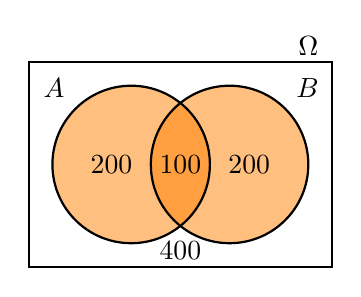
\begin{tikzpicture}[thick,
                    set/.style = {circle,
                                minimum size = 2cm,
                                fill=orange,
                                opacity=0.5}]
                    \draw [draw=black] (-1.3,-1.3) rectangle (2.55,1.3);
                    % Set A
                    \node[set,label={135:$A$}] (A) at (0,0) {};
                    % Set B
                    \node[set,label={45:$B$}] (B) at (1.25,0) {};
                    % Circles outline
                    \draw (0,0) circle(1cm);
                    \draw (1.25,0) circle(1cm);
                    % Set intersection label
                    \node at (0.625,0) {100};
                    \node at (-0.25,0) {200};
                    \node at (1.5,0) {200};
                    \node at (0.625,-1.1) {400};
                    \node at (2.25,1.5) {$\Omega$};
                \end{tikzpicture}
            \end{center}
            Hay 100 personas que son exitosas y están radicadas en el extranjero
        \item por lo menos una.\e\\
            En el diagrama podemos ver que hay 400 personas que no lograron ninguna de las dos, así que son $500(=900-400)$ aquellas que al menos lograron una.\e
        \item no más de una.\e\\
            Este grupo está conformado por las 200 personas que son exitosas pero no están en el extranjero y por las 200 personas radicadas en el extranjero pero no exitosas. Por lo tanto, hay 400 personas en total.
    \end{enumerate}
        %\item Un experimento aleatorio tiene tres resultados posibles: $a,b$ y $c$, con probabilidades $p,p^2$ y $p$ respectivamente. Hallar justificando apropiadamente el/los valores válidos de $p$.\e\\
    Tenemos que el espacio muestral es\[\Omega=\{a,b,c\}\]
    Entonces, por axioma 3:\begin{align*}
        P(\Omega)=1&=p(a)+p(b)+p(c)=p+p^2+p\\
        &\to p^2+2p-1=0\\
        &\to p=-1\pm\sqrt{2} 
    \end{align*}
    Sin embargo, $-1-\sqrt{2}$ implica una probabilidad negativa con lo cual\[p=-1+\sqrt{2}\]
        %\item Una caja tiene 10 bolas numeradas del 1 al 10. Una bola se elige al azar y una segunda bola se elige de las 9 restantes. Encontrar la probabilidad de que los números de las 2 bolas difieran en 2 o más.\e\\
    La primera bola puede ser cualquiera de las 10 en la caja mientras que la segunda es una entre nueve, por ende, hay \[10\cdot9=90\text{ casos totales}\]
    Para determinar los casos favorables, se puede pensar de la siguiente forma: Si saco 1 o 10, tengo 8 bolas que cumplen lo pedido
    \begin{center}
        $B_1=1\to B_2=i,\quad i=3,4,5,6,7,8,9,10$\\
        $B_1=10\to B_2=j,\quad j=1,2,3,4,5,6,7,8$ 
    \end{center}
    Mientras que con los otros números sólo tengo 7 opciones favorables ya que su anterior y siguiente no son válidos. Ej:\[B_1=5\to B_2=k,\quad k=1,2,3,7,8,9,10\]
    Teniendo en cuenta esto hay\[8\cdot7+2\cdot8=72\text{ casos favorables}\]
    Por lo tanto, sea $A=$ las bolas difieren en 2 o más, se tiene que\[P(A)=\frac{72}{90}\]
    También se podría haber pensado que\[P(A)=1-P(A^c)\]
    En donde $A^c$ contempla los casos en donde las bolas difieren en 1. Nuevamente, hay que separar de la siguiente manera: Si saco 1 o 10, la siguiente debe ser 2 o 9 respectivamente, para el resto hay 2 opciones. Entonces,
    \[P(A)=1-\frac{2\cdot1+8\cdot2}{90}=1-\frac{18}{90}=\frac{72}{90}\]
        %\item Se carga un dado de manera que los números pares tienen el doble de probabilidad de salir que los impares; los pares son igualmente probables entre sí, y lo mismo sucede con los impares. Se arroja el dado una vez. Hallar la probabilidad que:
    \begin{enumerate}
        \item Aparezca un número par.\e\\
            Tenemos que los impares son la mitad de probables que los pares. Si consideramos los eventos
            \begin{center}
                $A=$ sale un número par\\
                $B=$ sale un número impar
            \end{center}
            Entonces\[P(A)=2P(B)\]
            Además, el espacio muestral es\[\Omega=\{1,2,3,4,5,6\}\]
            y se sabe que\[A=\{2,4,6\}\qquad B=\{1,3,5\}\]
            Por el axioma 3\[P(A)=p(2)+p(4)+p(6)\qquad P(B)=p(1)+p(3)+p(5)\]
            Y como cada par e impar tienen la misma probabilidad entre sí\[P(A)=6c\qquad P(B)=3c\]
            Al ser $A$ y $B$ disjuntos, por la propiedad 1\[P(\Omega)=P(A\cup B)=P(A)+P(B)=9c=1\to c=\frac{1}{9}\]
            Por lo tanto\[P(A)=6\cdot\frac{1}{9}=\frac{6}{9}\]
        \item Aparezca un número impar.
            \[P(B)=3\cdot\frac{1}{9}=\frac{3}{9}\]
        \item Aparezca un número primo impar.\e\\
            Los números primos impares que pueden salir en un dado son 3 y 5. Como los impares son igual de probables y $P(B)=\frac{3}{9}\to p(1)=p(3)=p(5)=\frac{1}{9}$\[\to p(3)+p(5)=\frac{2}{9}\]
    \end{enumerate}
    \end{enumerate}
\end{document}